\documentclass[a4paper,11pt]{scrartcl}

% packages
\usepackage[ngerman]{babel}
\usepackage{graphicx}
\usepackage{url}
\usepackage{hyperref}
\usepackage{apacite}
\usepackage{tabularx}
\usepackage{listings}
\usepackage{fontspec}
    \setmainfont{Vollkorn}
    \setsansfont{Lato}
    \setmonofont{Inconsolata}
\usepackage[htt]{hyphenat}

% global options
\renewcommand{\baselinestretch}{1.25}
\pagestyle{headings}

% listing options
\lstset{basicstyle=\small\ttfamily,captionpos=b}
\renewcommand\lstlistlistingname{Verzeichnis der Codebeispiele}
\renewcommand\lstlistingname{Codebeispiel}

% macro definitions for references
\newcommand{\secref}[1]{{Abschnitt \ref{#1} \textit{\nameref{#1}}, Seite \pageref{#1}}}
\newcommand{\imgref}[1]{{Abbildung \ref{#1}, Seite \pageref{#1}}}
\newcommand{\tblref}[1]{{Tabelle \ref{#1}, Seite \pageref{#1}}}
\newcommand{\lstref}[1]{{Codebeispiel \ref{#1}, Seite \pageref{#1}}}

\begin{document}

\author{Patrick Bucher}
\title{px: PEAX Command Line Client}
\subtitle{Wirtschaftsprojekt, Herbstsemester 2019}
\date{\today}
\maketitle

\section*{Abstract}

Lorem ipsum dolor sit amet \cite[p. 99]{unixart}, consetetur sadipscing elitr \cite[p. 101]{cleanarch}, sed diam nonumy eirmod tempor invidunt ut labore et dolore magna aliquyam erat, sed diam voluptua. At vero eos et accusam et justo duo dolores et ea rebum. Stet clita kasd gubergren, no sea takimata sanctus est Lorem ipsum dolor sit amet \cite[p. 99]{testing}. Lorem ipsum dolor sit amet, consetetur sadipscing elitr, sed diam nonumy eirmod tempor invidunt ut labore et dolore magna aliquyam erat, sed diam voluptua \cite[p. 88]{unixphil}. At vero eos et accusam et justo duo dolores et ea rebum. Stet clita kasd gubergren, no sea takimata sanctus est Lorem ipsum dolor sit amet \cite[p. 23]{gopl}.

\newpage

\tableofcontents
\newpage

\section{Problemstellung}

\subsection{Analyse des Projektauftrags}

Die Umgebung der PEAX API einerseits

\subsubsection{Endpoints}

Eine RESTful-API besteht aus einer Reihe sogenannter \textit{Endpoints}, d.h Pfade zu Ressourcen, die abgefragt und/oder manipuliert werden können.

\subsubsection{HTTP-Methoden}

Ein Endpoint kann über eine oder mehrere HTTP-Methoden angesprochen werden \cite[Abschnitt 4.3]{RFC7231}. Im Kontext der PEAX API sind folgende Methoden relevant:

\begin{itemize}
	\item \texttt{GET}
	\item \texttt{HEAD}
	\item \texttt{POST}
	\item \texttt{PUT}
	\item \texttt{DELETE}
	\item \texttt{OPTIONS}
	\item \texttt{PATCH} \cite{RFC5789}
\end{itemize}

\subsubsection{HTTP Status-Codes}

Eine Antwort auf eine HTTP-Anfrage enthält jeweils einen Status-Code \cite[Abschnitt 6]{RFC7231}. Bei der PEAX API werden u.a. folgende Status-Codes häufig verwendet:

\begin{itemize}
	\item \texttt{200 OK}: Die Anfrage hat funktioniert.
	\item \texttt{201 Created}: Die Anfrage hat funktioniert, und dabei wurde eine neue Ressource erzeugt.
	\item \texttt{204 No Content}: Die Anfrage konnte ausgeführt werden, liefert aber keinen Inhalt zurück (etwa in einer Suche mit einem Begriff, zu dem keine Ressource gefunden werden kann).
	\item \texttt{204 Partial Content}: Der zurückgelieferte Payload repräsentiert nur einen Teil der gefundenen Informationen. Wird etwa beim Paging eingesetzt.
	\item \texttt{400 Bad Request}: Die Anfrage wurde fehlerhaft gestellt (ungültige oder fehlende Feldwerte).
	\item \texttt{401 Unauthorized}: Der Benutzer ist nicht autorisiert, d.h. nicht eingeloggt im weitesten Sinne.
	\item \texttt{403 Forbidden}: Der Benutzer ist zwar eingeloggt, hat aber keine Berechtigung mit der gewählten Methode auf die jeweilige Resource zuzugreifen.
	\item \texttt{404 Not Found}: Die Resource wurde nicht gefunden; deutet auf eine fehlerhafte URL hin.
	\item \texttt{405 Method Not Allowed}: Die Resource unterstützt die gewählte Methode nicht.
	\item \texttt{415 Unsupported Media Type}: Das Format des mitgelieferten Payloads wird nicht unterstützt. In der PEAX API sind dies etwa Dokumentformate, die beim Hochladen nicht erlaubt sind (z.B. \texttt{.exe}-Dateien).
	\item \texttt{500 Internal Server Error}: Obwohl die Anfrage korrekt formuliert und angenommen worden ist, kam es bei der Verarbeitung derselben zu einem serverseitigem Fehler.\footnote{In der PEAX API kommt es gelegentlich zu solchen Fehlern, die stattdessen mit dem Status \texttt{400 Bad Request} und einer aussagekräftigen Fehlermeldung beantwortet werden müssten. Wird z.B. bei der Einlieferung von Dokument-Metadaten eine syntaktisch fehlerhafte IBAN mitgegeben, tritt der Fehler erst bei der internen Verarbeitung, und nicht schon bei der Validierung der Anfrage auf. Hier besteht Handlungsbedarf aufseiten der Backend-Entwicklung.}
	\item \texttt{380 Unknown}: Dieser Status ist nicht Teil der HTTP-Spezifikation, wird aber nach einem Login-Versuch verwendet, wenn eine Zwei-Faktor-Authentifizierung (SMS, One Time Password) verlangt wird, und ist somit für die vorliegende Arbeit von hoher Relevanz.
\end{itemize}

\subsubsection{Umgebungen}
\subsubsection{Arten von Parametern}
\subsubsection{Benutzer}
\subsubsection{Betriebssysteme}
\subsubsection{Shells} 

\subsection{Ausgangslage und Vorleistungen}

Das Projekt \texttt{px} wurde bereits am 11. Juni 2019 auf dem GitLab von PEAX erstellt\footnote{\url{https://gitlab.peax.ch/peax3/px}}. Als erstes wurde eine CI-Pipeline bestehend aus den Schritten `build` und `test` erstellt. Die Pipeline wurde mittels eines Dummy-Tests überprüft, der einmal erfolgreich durchlaufen und einmal scheitern sollte, um einen Positiv- und einen Negativtest durchführen zu können.

Es wurde eine Hallo-Welt-Programm im \texttt{cmd}-Unterverzeichnis \cite[p. 293]{gopl} erstellt, welches dazu diente, die Kompilierung für verschiedene Plattformen zu testen. Obwohl Go-Programme mittels `go build` kompiliert werden können und keine weitere Build-Konfiguration benötigen, wurde ein \texttt{Makefile} erstellt, das Builds für verschiedene Plattformen im \texttt{build}-Unterverzeichnis erstellt, also z.B. \texttt{build/windows/px.exe} für Windows oder \texttt{build/linux/px} für Linux.

Das \texttt{Makefile} wurde später um ein \texttt{release}-Target erweitert, womit die kompilierten Artefakte jeweils in eine Zip-Datei verpackt werden, die den aktuellen Versionstag (z.B. \texttt{v0.0.3}\footnote{\url{https://semver.org/}}) im Dateinamen enthält.

Das Target \texttt{coverage} führt die Testfälle durch, misst die Testabdeckung und generiert eine HTML-Ausgabe des getesteten Codes. Rote Zeilen sind nicht durch einen Testfall abgedeckt, grüne Zeilen hingegen schon. \cite[Kapitel 11.3]{gopl}

Weiter sind bis am 31. Juli 2019 folgende Features implementiert worden:

\begin{description}
	\item[\texttt{px help}] zeigt eine einfache Hilfeseite auf der Kommandozeile an.
	\item[\texttt{px login}] führt einen Loginversuch mit den angegebenen Credentials durch. Benutzername und Passwort können entweder als Kommandozeilenparameter oder mittels interaktiver Eingabe (\texttt{stdin}) entgegengenommen werden. Im letzteren Fall wird das eingegebene Passwort nicht angezeigt, was mit einem externen SSH-Terminal-Modul\footnote{\url{https://godoc.org/golang.org/x/crypto/ssh/terminal\#Terminal.ReadPassword}} erreicht wird. Bei einem erfolgreichen Login-Versuch werden \texttt{access\_token} und \texttt{refresh\_token} aus dem Response-Payload gelesen und im \texttt{\$HOME}-Verzeichnis des jeweiligen Betriebssystem-Benutzers in eine JSON-Datei namens \texttt{.px-tokens} abgespeichert.
	\item[\texttt{px logout}] löscht ein Token-Paar für eine bestimmte Umgebung. Pro Umgebung kann es zu jedem Zeitpunkt nur ein aktives «Login», d.h. Token-Paar geben. Es besteht auch die Möglichkeit, sämtliche Tokens auf einmal zu löschen. Hierbei wird \texttt{\$HOME/.px-tokens} nicht gelöscht, sondern nur das Property \texttt{tokens} geleert. (Die Datei enthält ein Initialisierungsdatum, das nicht verlorengehen soll.)
	\item[\texttt{px upload}] lädt eine Datei (z.B. PDF) auf das PEAX-Portal hoch. Diese Funktionalität wurde eingebaut, um die Funktionsweise von \texttt{px} vor dem Ideation-Gremium zu demonstrieren\footnote{Die hochgeladene Datei erschien Sekunden später im Web-Portal, was die Anwesenden von der Funktionsweise überzeugte}.
\end{description}

Für die Evaluierung des Prototypen werden zudem die Anzahl Aufrufe und das Datum des letzten Aufrufs von \texttt{px} in eine JSON-Datei \texttt{\$HOME/.px-usage} geschrieben.

Insgesamt wurden ca. 20 Arbeitsstunden in den Prototyp investiert. Ein grosser Teil des Codes kann für die Weiterentwicklung übernommen werden, muss jedoch umstrukturiert werden. So ist zuviel Logik im Hauptmodul \texttt{cmd/px.go}, die zwecks Wiederverwendbarkeit in das Library-Modul \texttt{px} überführt werden soll.

\newpage

\section{Stand der Praxis}

\subsection{Ansprechen der PEAX API}

TODO: Problematik mit Postman, cUrl, httpie beschreiben

\subsection{Kommandozeilenprogramme}

TODO: docker, oc und git beschreiben

\newpage

\section{Ideen und Konzepte}

TODO: swiss army knive \cite[p. 290]{gopl} für CLI

TODO: token storage (sicher und unsicher)

TODO: automatisches Retry

\newpage

\section{Methoden}

\subsection{Teststrategie}

Wie im Vorsemester im Modul \textit{Software Testing} eingeübt, sollen die \textit{Agile Test Quadrants} (\imgref{fig:agile-testing-quadrants}) als Grundlage zur Erarbeitung einer Teststrategie dienen \cite[p. XX]{agiletest}.

\begin{figure}
	\centering
	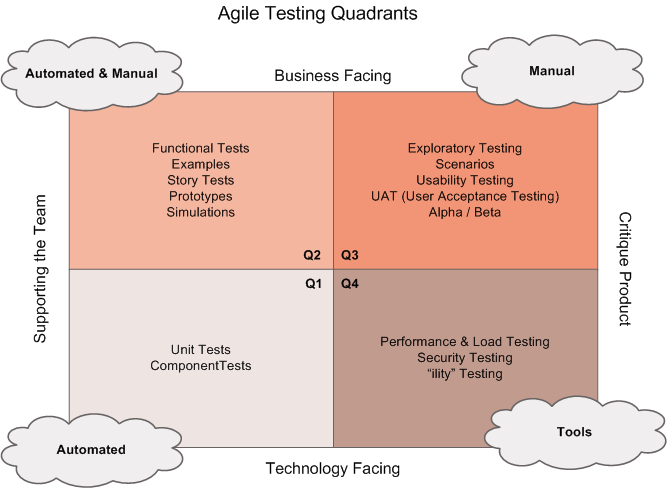
\includegraphics[width=\linewidth]{pics/agile-testing-quadrants.png}
	\caption{\textit{Agile Testing Quadrants} nach Lisa Crispin (\url{https://lisacrispin.com/2011/11/08/using-the-agile-testing-quadrants/})}
	\label{fig:agile-testing-quadrants}
\end{figure}

\newpage

\section{Realisierung}

\newpage

\section{Evaluation und Validierung}

\subsection{Rückmeldungen von Entwicklern}

\subsubsection{Sprint 1}

\begin{itemize}
    \item \textsc{Michael Buholzer} wünscht sich Erfolgs- und Vollzugsmeldungen nach dem Login oder dem Upload eines Dokuments.
    \begin{itemize}
        \item \texttt{stdout} sollte grundsätzlich «sauber» bleiben, d.h. frei von unnötigen Ausgaben, die ein nachgelagertes Programm wieder herausfiltern müsste. Eine wichtige Maxime von UNIX-Programmen lautet: \textit{«Expect the output of every program to become the input to another, as yet unknown, program.»} \cite[p. 3]{unixtimesharing}. Siehe dazu auch \textit{Rule of Silence} \cite[p. 20]{unixart} und \textit{Silence is Golden} \cite[p. 111]{unixphil}.
        \item \texttt{stderr} wird nicht nur als Ausgabekanal für Fehlermeldungen verwendet, sondern für Meldungen allgemein. Für Vollzugsmeldungen wäre \texttt{stderr} vorzuziehen.
        \item Da \texttt{stderr} in \texttt{px} bisher grundsätzlich für Fehlermeldungen verwendet wird, sollen Erfolgsmeldungen über ein zusätzliches Flag \texttt{-verbose}/\texttt{-v} aktiviert werden müssen.
        \item Bei anderen Anwendungsfällen signalisiert die Ausgabe des Payloads auf \texttt{stdout} den Erfolg der Operation. Beim Dokument-Upload besteht dieser beispielsweise aus der generierten UUID des hochgeladenen Dokuments.
    \end{itemize}
\item \textsc{Patrick Roos} sieht die Möglichkeit, \texttt{px} auch zur Handhabung der \textit{Vault Secrets}\footnote{\url{https://docs.ansible.com/ansible/latest/user_guide/vault.html}} (Verschlüsselung und Entschlüsselung von Benutzernamen, Passwörtern etc. zu verwenden.
    \begin{itemize}
        \item Im Arbeitsalltag von PEAX stellt die Handhabung von Vault Secrets tatsächlich eine teils mühsame und langwierige Aufgabe dar. Hier besteht durchaus Automatisierungsbedarf.
        \item \texttt{px} ist als «skriptbare» Anwendung für die PEAX API konzipiert und so potenziell für jeden PEAX-Anwender einsetzbar.
        \item Die Verwaltung und Verwendung von Vault Secrets ist hingegen eine Aufgabe im DevOps-Bereich und betrifft nur interne Entwickler bei PEAX.
        \item Eine der obersten Maximen von UNIX lautet: \textit{«Make each program do one thing well. To do a new job, build afresh rather than complicate old programs by adding new ‹features.›} \cite[p. 3]{unixtimesharing} Die Verwaltung von Vault Secrets und das Ansprechen der PEAX API sind klar zwei verschiedene Sachen und somit nicht «one thing». Die genannte Idee muss also anderweitig weiterverfolgt werden.
    \end{itemize}
\end{itemize}

\newpage

\section{Ausblick}

TODO: OpenSource, auf dem Laufenden halten, unterschiedliche API-Versionen, wie weiter?

\newpage

\section{Anhang}

\subsection{Technologie-Evaluation}

- Vorgabe: PEAX API (RESTful)

\subsubsection{Programmiersprache}

Anforderungen:

\begin{description}
    \item[Installation] Die Software soll sich einfach installieren lassen.
    \item[Umgebung] Es dürfen keine besonderen Anforderungen an die Umgebung gestellt werdenm auf der \texttt{px} läuft.
    \item[Plattformen] Die Software soll auf allen gängigen Betriebssystemen (Windows, mac OS, Linux) lauffähig sein.
    \item[Einheitlichkeit] Der Client soll überall die gleiche Befehlssyntax haben.
    \item[Performance] Ein Command Line Client soll in Skripten verwendet werden können, wodurch das Programm sehr oft in kurzem Zeitraum aufgestartet werden muss.
\end{description}

Java erfordert die lokale Installation einer JRE in der richtigen Version. Ausserdem werden Wrapper-Skripts benötigt (\texttt{java -jar px.jar} ist nicht praktikabel).

Python, Ruby, Perl und andere Skriptsprachen benötigen ebenfalls einen vorinstallierten Interpreter in der richtigen Version.

Zwar gibt es mit Mono eine Variante von .Net, die überall lauffähig ist, hier werden aber wiederum eine Laufzeitumgebung bzw. vorinstallierte Libraries benötigt.

Am besten geeignet sind kompilierte Sprachen (C, C++, Go, Rust, Nim). Mit einer statischen Kompilierung lässt sich das ganze Programm in eine einzige Binärdatei überführen, welches denkbar einfach zu installieren ist (Kopieren nach einem der Verzeichnisse innerhalb von \texttt{\$PATH}).

Für JavaScript gibt es mit QuickJS seit kurzem die Möglichkeit, JavaScript zu Binärdateien zu kompilieren. Dies funktioniert aber nicht auf allen Plattformen, ausserdem ist QuickJS noch experminentell und noch nicht für den produktiven Einsatz geeignet.

In die engere Auswahl kommen Go und Rust, da der Autor dieser Arbeit mit diesen Programmiersprachen bereits Erfahrungen im Studium machen konnte. (Mit C++ noch keine Erfahrungen gemacht. Mit C Erfahrungen gemacht, wodurch es als sehr aufwändig erscheint, einen HTTP-Client zu schreiben.)

\subsubsection{Go}

\begin{itemize}
    \item einfach zu lernen (wenige Keywords und Features), dafür keine Features wie Generics und map/filter/reduce
    \item gutes und übersichtliches Tooling
    \item Cross-Compilation ohne Zusatztools möglich
    \item Kompilierung zu statischen Binaries, die jedoch recht gross ausfallen (Prototyp: ca. 4 MB)
    \item Kompilierung extrem schnell
    \item umfassende und qualitativ hochwertige Standard Library, inkl. HTTP-Library
    \item persönlich bereits viel damit gearbeitet, positive Erfahrungen damit gemacht
    \item Error Handling aufwändig, führt aber zu sehr solidem, wenn auch repetitivem Code
    \item vergleichbare Software (\texttt{oc}: OpenShift Command Line Client, \texttt{docker}: Docker Command Line Client) ist ebenfalls in Go geschrieben und bei uns täglich erfolgreich im Einsatz
    \item fügt sich sehr gut in UNIX-Philosophie ein (Tooling, Libraries)
    \item Einfaches Interface für nebenläufige Programmierung (Goroutines und Channels)
    \item Performance im Bereich von Java, jedoch tieferer Memory-Footprint
\end{itemize}

\subsection{Rust}

\begin{itemize}
    \item viele Features, dafür aber schwer zu lernen (Lifetimes, Borrowing, siehe PCP)
    \item gutes und übersichtliches Tooling
    \item Kompilierung in statische Binaries, die relativ schlank ausfallen
    \item Kompilierung eher langsam
    \item Cross-Compilation benötigt Zusatztools
    \item wenig Erfahrung damit gesammelt
    \item Standard Library bewusst schlank gehalten, dafür viele externe Libraries benötigt
    \item extrem ausdrucksstarke Sprache mit starkem Typsystem
    \item diverse Rust-Utils erfolgreich persönlich im Einsatz (rg, bat, hexyl, battop)
    \item erstklassige Performance (im Bereich von C/C++)
\end{itemize}

\subsection{Libraries}

\newpage

\section{Einstiegsbeispiel}

\begin{lstlisting}[language=Go,caption={Some Go Code}]
package main

import (
	"fmt"
	"log"
	"os"

	"gopl.io/ch05/links"
)

// breadthFirst calls f for each item in the worklist.
// Any items returned by f are added to the worklist.
// f is called at most once for each item.
func breadthFirst(f func(item string) []string, worklist []string) {
	seen := make(map[string]bool)
	for len(worklist) > 0 {
		items := worklist
		worklist = nil
		for _, item := range items {
			if !seen[item] {
				seen[item] = true
				worklist = append(worklist, f(item)...)
			}
		}
	}
}

func crawl(url string) []string {
	fmt.Println(url)
	list, err := links.Extract(url)
	if err != nil {
		log.Print(err)
	}
	return list
}

func main() {
	// Crawl the web breadth-first,
	// starting from the command-line arguments.
	breadthFirst(crawl, os.Args[1:])
}
\end{lstlisting}

\newpage

\bibliographystyle{apacite}
\bibliography{document}
\newpage

\listoffigures
\addcontentsline{toc}{section}{Abbildungsverzeichnis}
\newpage

\listoftables
\addcontentsline{toc}{section}{Tabellenverzeichnis}
\newpage

\lstlistoflistings
\addcontentsline{toc}{section}{Verzeichnis der Codebeispiele}

\end{document}
